\section{Cartographie métier cible}
\label{sec:metier}

\subsection{Services, acteurs et processus}
La vue métier (figure~\ref{fig:metier}) organise le périmètre autour de cinq services rendus~: la demande et le renouvellement de la CNIE, la prise de rendez-vous, le suivi, l'identité numérique et l'authentification offerte aux fournisseurs accrédités. Le processus principal P0 se décompose en quatre sous-processus enchaînés~: SP1 pré-demande, contrôle des pièces et rendez-vous (nouveau)~; SP2 enrôlement au CEDI (à faire évoluer)~; SP3 production et personnalisation (conservé)~; SP4 notification, remise et activation de l'identité numérique (à faire évoluer). Un nouvel acteur apparaît~: l'\emph{agent instructeur}, qui traite à distance les dossiers que le contrôle automatique n'a pas pu trancher, ce qui déplace une partie de la charge des guichets vers un back-office mutualisé.

\begin{figure}[h]
\centering
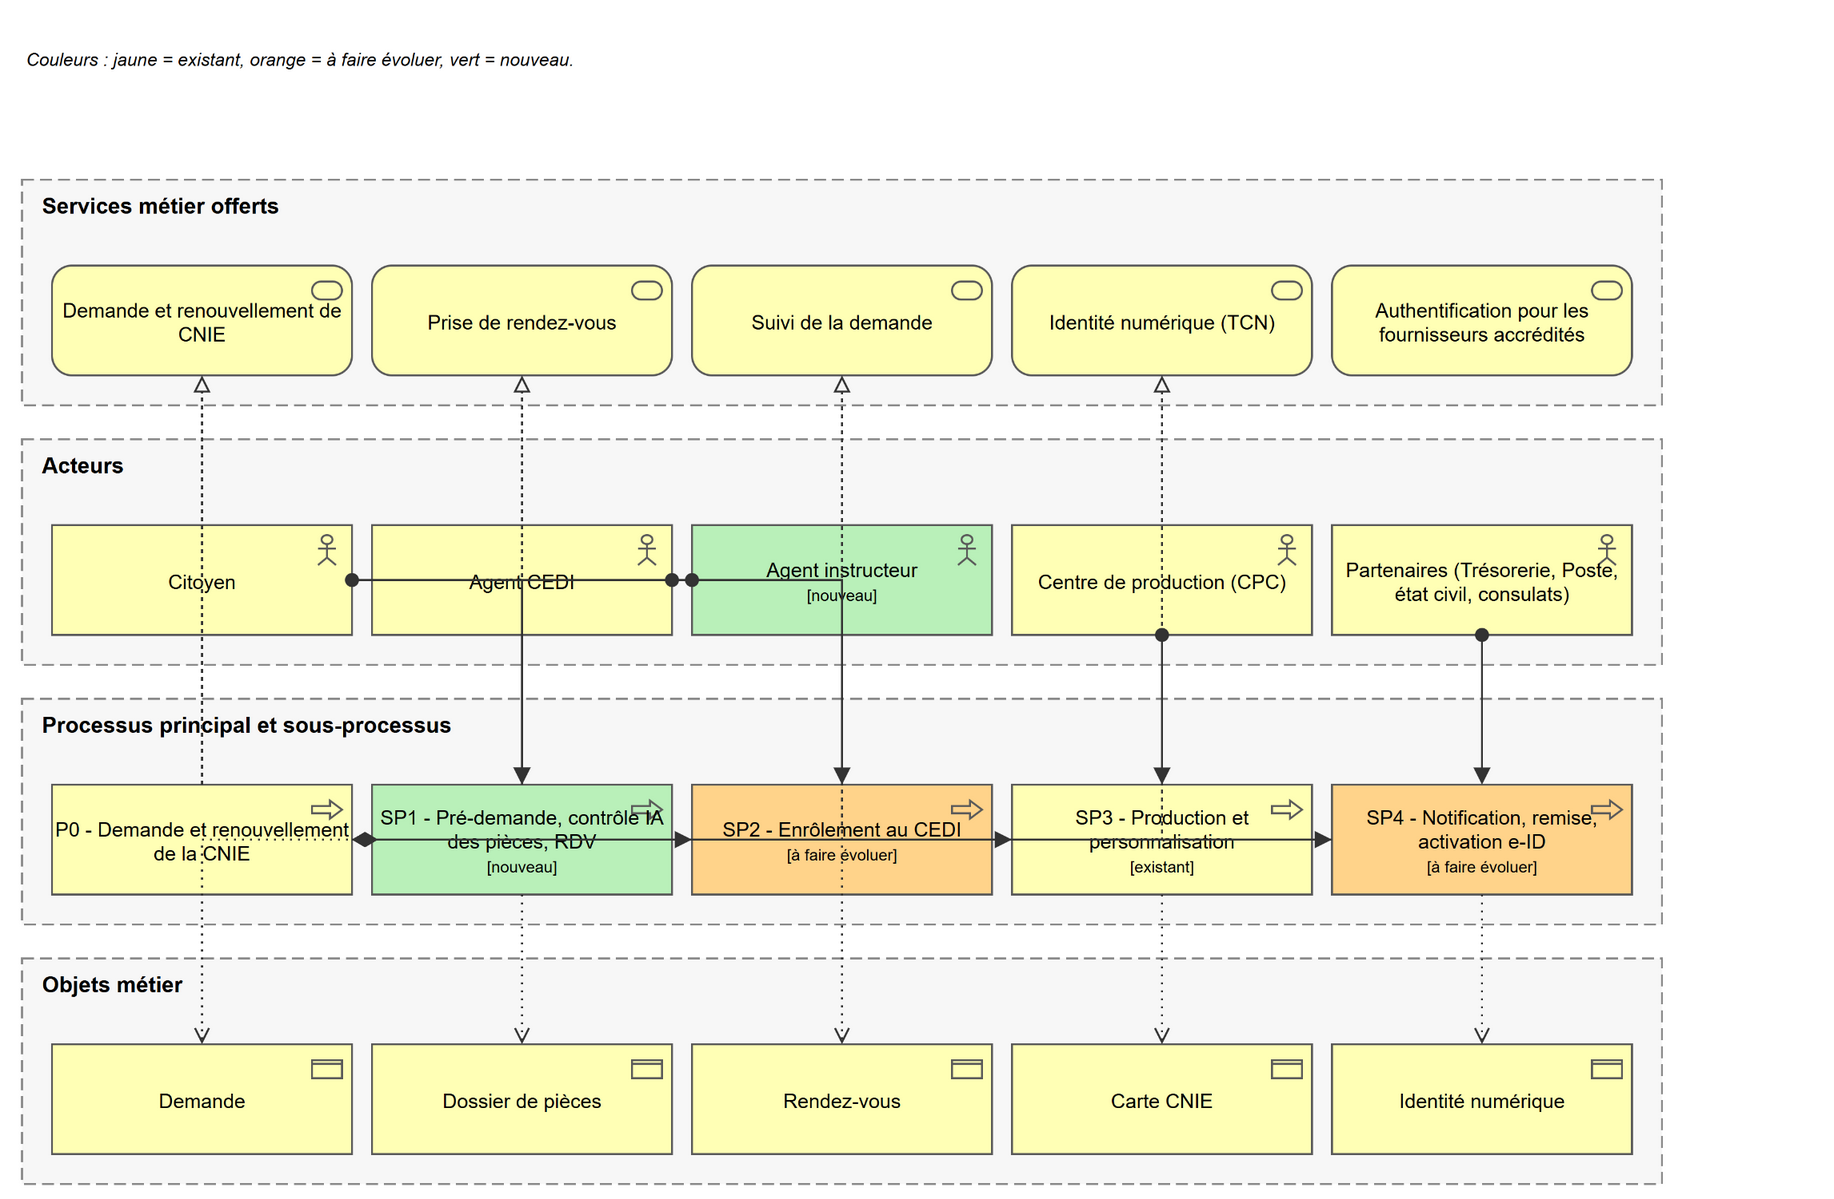
\includegraphics[width=\columnwidth]{archimate/V2_metier.png}
\caption{Vue métier cible~: services, acteurs, processus et objets métier.}
\label{fig:metier}
\end{figure}

\subsection{Le processus cible}
La figure~\ref{fig:bpmn-tobe} présente le processus P0 cible modélisé sous Blueworks Live. Par rapport à l'existant, six transformations sont introduites~:
\begin{enumerate}
  \item \textbf{Entrée par l'identité numérique}~: le citoyen déjà porteur d'une carte s'authentifie via la plateforme Tiers de Confiance et sa demande est pré-remplie à partir de la carte et de l'état civil (principe «~dites-le nous une fois~»).
  \item \textbf{Contrôle documentaire immédiat (IA-2)}~: les pièces téléversées sont analysées en quelques secondes~; un score de conformité oriente la demande vers la confirmation, vers une correction par le citoyen ou vers l'instruction humaine. Le dossier incomplet est détecté avant le déplacement, et non après.
  \item \textbf{Paiement intégré}~: l'e-timbre est vérifié en ligne au moment de la demande, sans ressaisie de code.
  \item \textbf{Créneaux recommandés (IA-4)}~: la prévision d'affluence propose les créneaux les moins chargés, avec convocation par QR code et rappels automatiques.
  \item \textbf{Enrôlement allégé et sécurisé (IA-3)}~: au CEDI, l'agent scanne la convocation et ne réalise que la capture biométrique~; la vérification d'unicité et la détection de fraude sont exécutées en temps réel et toute alerte est routée vers l'instructeur.
  \item \textbf{Remise au choix et activation}~: la carte est retirée au centre ou livrée à domicile avec authentification du porteur, puis la carte numérique est activée dans l'application «~Mon e-ID~», ce qui clôt le processus sur un citoyen immédiatement équipé pour les services en ligne.
\end{enumerate}

\begin{sidewaysfigure*}
\centering
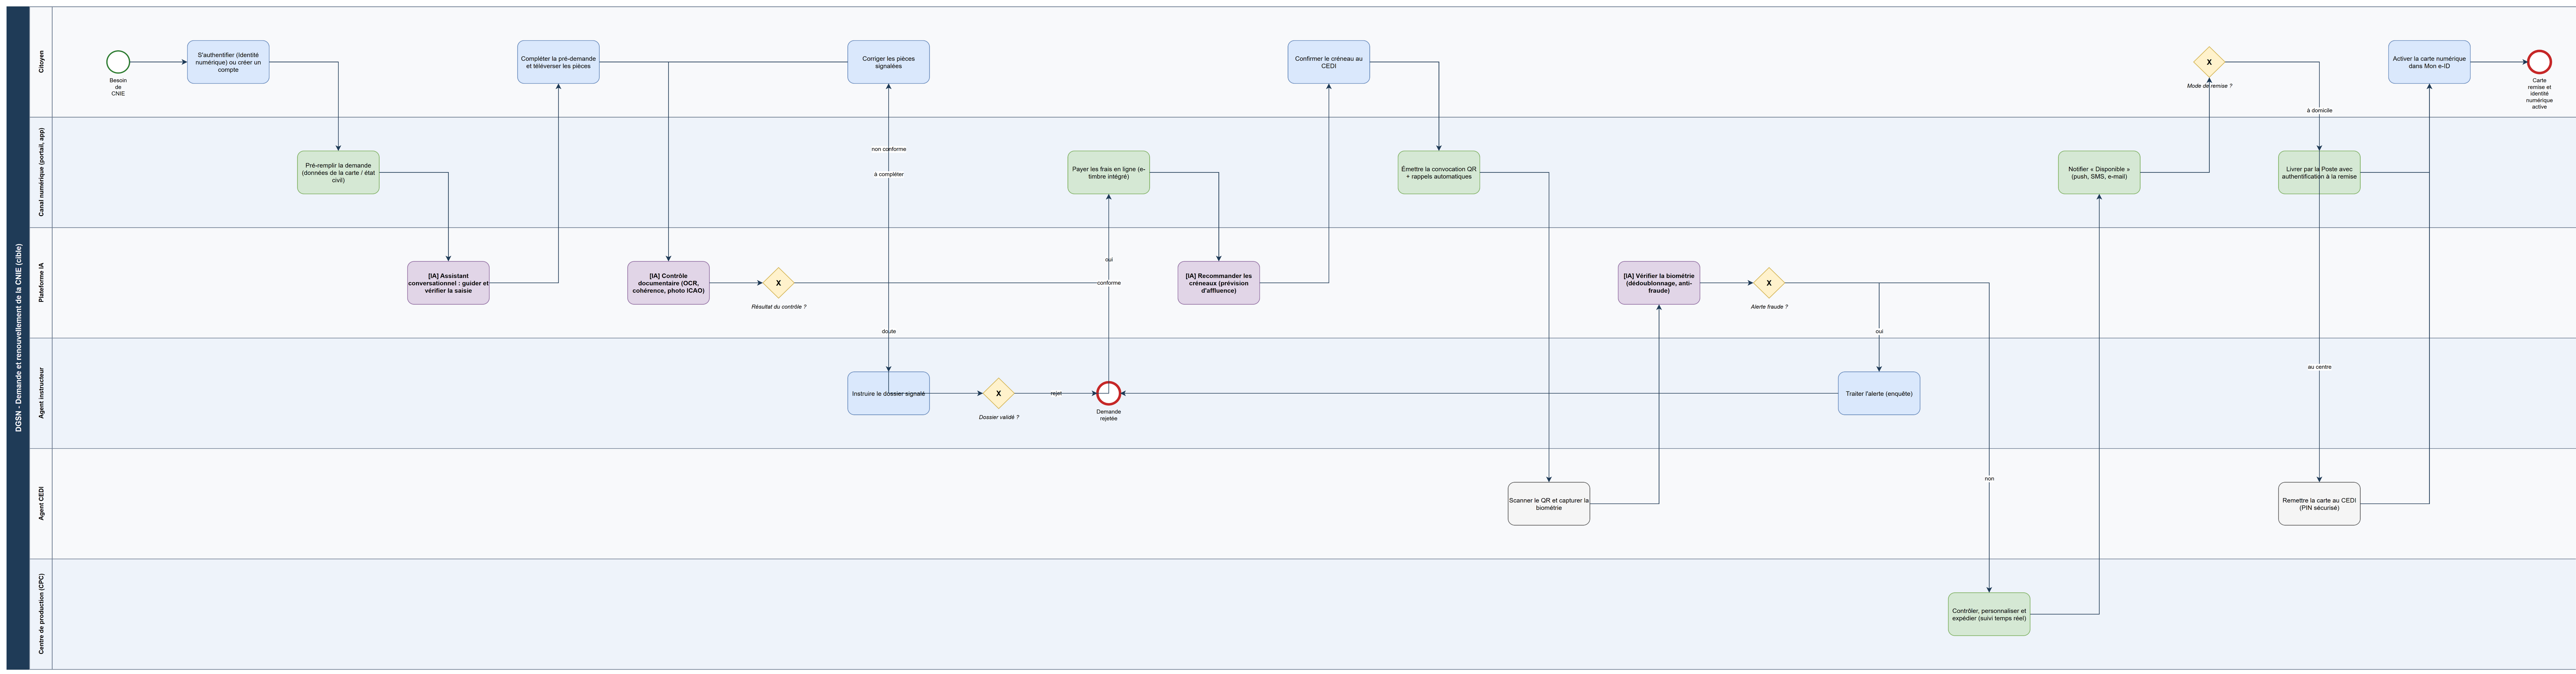
\includegraphics[width=\textwidth]{bpmn/P0_demande_cnie_tobe.png}
\caption{Processus P0 cible (to-be)~: les tâches en violet sont réalisées par la plateforme d'IA~; deux nouveaux couloirs apparaissent (plateforme IA, agent instructeur).}
\label{fig:bpmn-tobe}
\end{sidewaysfigure*}

\subsection{Indicateurs de performance du processus}
Pour piloter la transformation, nous proposons de suivre~: le taux de dossiers conformes au premier contrôle, le taux de dossiers incomplets constatés au guichet (cible $<$~5~\%), le délai médian entre la demande et la remise, le temps moyen de passage en centre, le taux d'occupation des créneaux par centre, le nombre d'alertes de fraude confirmées, et le taux d'activation de l'identité numérique à la remise. Ces indicateurs alimentent la zone de pilotage décrite dans la cartographie fonctionnelle.
